\pagenumbering{gobble}
\newgeometry{top=7cm, bottom=7cm}

\begin{center}
\Huge{\textbf{Note di calcolabilità}}\\
\vspace{10pt}
\large{\faGlobe\hspace{5pt}\texttt{matteogiorgi.github.io}}\\
\vspace{5\baselineskip}
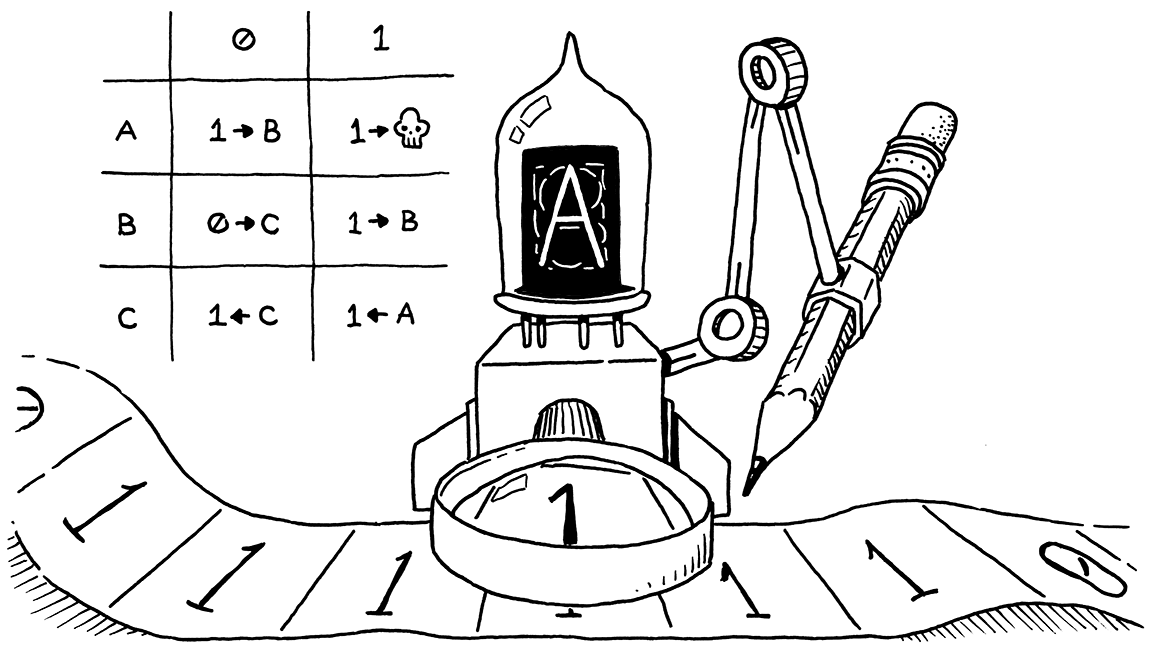
\includegraphics[width=0.8\textwidth]{../assets/machine.png}\\
\end{center}

\newpage
\restoregeometry
\pagenumbering{roman}
\renewcommand{\abstractname}{Info\hspace{5pt}\faPencil}

\begin{abstract}
Queste note sono state redatte dal sottoscritto durante le lezioni del corso di \textit{Elementi di calcolabilità e complessità} tenute dal prof. Pierpaolo Degano per il Corso di Laurea in Informatica presso l'Università di Pisa, anno accademico 2019-2020.

Il materiale usato per la stesura, oltre alle note distribuite dal professore, comprende, in maniera più o meno estensiva, riferimenti ai seguenti testi:

\begin{itemize}[itemsep=-7pt]
\item \textit{M. Sipser - Introduction to the theory of computation}
\item \textit{R.G. Taylor - Models of computation and formal languages}
\item \textit{N.J. Cutland - Computability, introduction to recursive function theory}
\item \textit{S.B. Cooper - Computability theory}
\item \textit{A. Bernasconi, B. Codenotti - Introduzione alla complessità computazionale}
\item \textit{G. Ausiello, F. D'Amore, G. Gambosi - Linguaggi, modelli, complessità}
\end{itemize}
\end{abstract}

\newpage
\tableofcontents

\newpage
\pagenumbering{arabic}
